% Manuscript frontmatter uses the standard elsarticle class and its public API.
% Class documentation: https://ctan.org/pkg/elsarticle
\documentclass[preprint,12pt,authoryear]{elsarticle}
\usepackage{amsmath,amssymb}
\usepackage{iftex}
\ifPDFTeX
  \usepackage[T1]{fontenc}
  \usepackage[utf8]{inputenc}
  \usepackage{textcomp}
\else
  \usepackage{unicode-math}
  \defaultfontfeatures{Ligatures=TeX}
\fi
\usepackage{lmodern}
\usepackage{xcolor}
\usepackage{microtype}
\usepackage{longtable,booktabs,array,calc}
\usepackage{etoolbox}
\usepackage{footnotehyper}
\makesavenoteenv{longtable}
\usepackage{xurl}
\usepackage[hidelinks,unicode]{hyperref}
\usepackage{bookmark}
\urlstyle{same}
\setcounter{secnumdepth}{3}
\providecommand{\tightlist}{\setlength{\itemsep}{0pt}\setlength{\parskip}{0pt}}
\makeatletter
\patchcmd\longtable{\par}{\if@noskipsec\mbox{}\fi\par}{}{}
% Suppress the submission-to-Elsevier footer present in older class releases.
\def\ps@pprintTitle{\let\@oddhead\@empty\let\@evenhead\@empty
  \def\@oddfoot{\hfil\thepage\hfil}\let\@evenfoot\@oddfoot}
\makeatother
\usepackage{tikz}
\usetikzlibrary{arrows.meta,positioning,fit,backgrounds}
\usepackage{needspace}
\definecolor{ink}{gray}{0.15}
\definecolor{light}{gray}{0.96}
\setlength{\emergencystretch}{3em}
\setlength{\LTpre}{6pt}
\setlength{\LTpost}{6pt}
\AtBeginEnvironment{longtable}{\footnotesize}
\tikzset{box/.style={draw=ink,rounded corners=2pt,fill=light,align=center,font=\footnotesize\sffamily,minimum height=10mm,inner sep=5pt},flow/.style={-{Stealth[length=2mm]},thick,draw=ink}}
\hypersetup{pdftitle={The Orchestrator: A Lifecycle Architecture for
Self-Developing, Self-Operating, and Self-Improving Agentic
Systems},pdfauthor={Timothy O'Brien},
  pdfkeywords={agentic systems, ontology evolution, self-adaptive
systems, semantic contracts, delegated intelligence, lifecycle
governance},pdflang={en-US}}
\begin{document}
\begin{frontmatter}
\title{The Orchestrator: A Lifecycle Architecture for Self-Developing,
Self-Operating, and Self-Improving Agentic Systems\tnoteref{preprint}}
\tnotetext[preprint]{Preprint; not peer reviewed.
  Version 0.2.1, 9 October 2026.}
\author{Timothy O'Brien\fnref{orcid}}
\fntext[orcid]{ORCID: \href{https://orcid.org/0009-0001-2589-347X}{0009-0001-2589-347X}.}
\begin{abstract}
\small
Agentic systems that perform delegated work also need a controlled way
to change the concepts and capabilities on which that work depends. This
paper proposes a reference architecture organized around DEVELOP,
OPERATE, and IMPROVE, coordinated by a durable orchestration layer. Its
central unit of deployment is an immutable operating bundle binding
executable capabilities to a versioned semantic snapshot, authority
policy, evaluation suite, and state compatibility contract. Operational
observations challenge the approved model through discrepancy reports,
candidate ontology branches, capability development, independent
validation, and explicit promotion. The architecture specifies lifecycle
transitions, typed handoff contracts, semantic impact obligations, and
deployment fencing. A worked example shows how an ontology change can
broaden an action's eligibility without changing policy text, while an
independent action gate blocks the prohibited effect. Drawing on
autonomic computing, runtime models, ontology evolution, and governed
capability deployment, the paper connects semantic release identity to
authority review and distributed action enforcement. A conditional
invariant argument characterizes release integrity, action coherence,
and proposal isolation under stated trust assumptions. The contribution
is an architectural synthesis supported by illustrative schemas and a
falsifiable evaluation design; operational effectiveness and the
additional value of ontology-based controls remain unevaluated.
\end{abstract}
\begin{keyword}
\small
agentic systems \sep ontology evolution \sep self-adaptive
systems \sep semantic contracts \sep delegated
intelligence \sep lifecycle governance
\end{keyword}
\end{frontmatter}
\pagestyle{plain}
\section{Introduction}\label{introduction}

An agent that can complete a task is not necessarily a system that can
maintain the capability to complete that task over time. Procedures
become inadequate, observations challenge existing categories, tools
change, and the interpretation of a policy may shift when its vocabulary
changes. Continuous operation therefore creates a second problem: how to
evolve the system without making its operating assumptions untraceable
or allowing its effective authority to expand silently.

Consider a courier in a fantasy library. It transports objects
classified as library artifacts. A newly encountered lantern speaks,
chooses its destination, and objects to being packed. The courier's
model distinguishes artifacts, rooms, and transport procedures, but
contains no category for an artifact with preferences. Calling the
encounter simply a failed tool call misses the representational problem.
Allowing the courier to invent and adopt a new authoritative category
during the same task risks changing the meaning of its permissions.
Freezing the model indefinitely leaves the system unable to learn from
recurring encounters.

The research question is: \textbf{Can autonomous software systems be
organized into distinct development, operation, and improvement
functions, coordinated through a shared, versioned ontology, to support
continuous evolution while preserving semantic consistency,
configuration reproducibility, and controlled authority?} This paper
gives a reference architecture and a qualified answer: such a separation
can specify enforceable release and action boundaries, provided that the
semantic dependencies are actually pinned and the boundaries are
mediated by trusted services. It cannot ensure that the model describes
the world correctly or that an agent recognizes every unfamiliar
situation.

We call the three functions DEVELOP, OPERATE, and IMPROVE. OPERATE
performs delegated work using approved capabilities. IMPROVE
investigates deficiencies and proposes changes. DEVELOP implements and
tests executable capabilities against an identified semantic snapshot.
An orchestrator coordinates their transitions and invokes independent
release controls. These are responsibilities, not a requirement to run
exactly three language models.

The paper makes four contributions as an architectural synthesis:

\begin{enumerate}
\def\labelenumi{\arabic{enumi}.}
\tightlist
\item
  A deployment contract binding semantics, capabilities, authority,
  evaluation, and state compatibility into an immutable operating
  bundle.
\item
  A lifecycle in which evidence can challenge production semantics
  through an explicit report, candidate branch, implementation,
  validation, and promotion sequence.
\item
  A semantic impact obligation that includes changes in policy
  denotation and capability applicability, even when policy and
  capability source files are unchanged.
\item
  A distributed deployment contract connecting approval to an exact
  bundle, an activation epoch, compatible state, and action-time
  enforcement.
\end{enumerate}

The contribution lies in specifying how established mechanisms interact
for delegated agentic work: what each transition binds, which authority
approves it, and which obligations remain at the point of action. The
following sections relate this contract to its architectural foundations
and define how its practical value could be tested.

\section{Positioning and research
method}\label{positioning-and-research-method}

\subsection{Prior architectural
foundations}\label{prior-architectural-foundations}

Autonomic computing already treats systems as entities that monitor and
adapt their own operation. MAPE-K separates monitoring, analysis,
planning, execution, and shared knowledge. DEVELOP/OPERATE/IMPROVE does
not replace that control model: OPERATE belongs largely to the managed
application; IMPROVE groups analysis and planning; DEVELOP supplies
artifacts used in adaptation; orchestration coordinates execution and
release. The mapping is many-to-many because monitoring and knowledge
management cut across the functions.
\href{https://doi.org/10.1109/MC.2003.1160055}{Kephart and Chess
(2003)}.

IBM's architectural blueprint also discusses orchestrated managers,
policy-based delegation, composed management functions, and shared
knowledge with common syntax and semantics. These provide the foundation
for treating coordination and semantic interpretation as shared
management responsibilities.
\href{https://users.cs.fiu.edu/~sadjadi/Teaching/Autonomic\%20Grid\%20Computing/CIS-6612-Summer-2006/AC-Blueprint-WhitePaper-V7.pdf}{IBM
(2005)}.

Architecture-based adaptation and models maintained during execution are
also established. Rainbow uses an external architecture-based adaptation
framework, while models@run.time addresses causally connected models
that guide executing systems. They establish the use of an explicit
runtime model and a separate adaptation layer.
\href{https://www.cs.cmu.edu/~able/publications/computer04/}{Garlan et
al.~(2004)}; \href{https://doi.org/10.1109/MC.2009.326}{Blair, Bencomo,
and France (2009)}.

Ontology evolution research has long examined changes, consistency,
dependent artifacts, and propagation. Git-backed RDF version control is
likewise established. These sources motivate treating an ontology branch
as an engineering artifact whose dependencies and propagation effects
require review.
\href{https://doi.org/10.1007/3-540-45810-7_27}{Stojanovic et
al.~(2002)}; \href{https://arxiv.org/abs/1805.03721}{Arndt et
al.~(2019)}.

The connection between semantic evolution and security is also older
than agentic software. Peldszus and colleagues describe semantic change
detection, co-evolution proposals, and security compliance analysis. Our
emphasis on authority affected by meaning changes is therefore an
application and integration of an existing concern.
\href{https://doi.org/10.1016/j.datak.2021.101907}{Peldszus et
al.~(2021)}.

\subsection{Closest contemporary
comparisons}\label{closest-contemporary-comparisons}

Three recent systems provide particularly close comparisons. Declarative
Lifecycle Management for Self-Adaptive Systems connects semantic
lifecycle descriptions to reconfiguration of managing-system components.
EvoOntology maintains a versioned schema/content/tool ontology layer,
uses operational trajectories to propose localized changes, and rejects
candidates that fail paired evaluation. Governed Capability Evolution
specifies compatibility checks and staged admission, monitoring,
withdrawal, and audit for versioned AI components.
\href{https://doi.org/10.1007/s10270-026-01358-w}{Kamburjan et
al.~(2026)}; \href{https://arxiv.org/abs/2609.15779v1}{Chong et
al.~(2026)}; \href{https://arxiv.org/abs/2604.08059v6}{Qin et
al.~(2026)}.

Further close comparisons include ontology-aware scientific tool
acquisition, a bounded-autonomy workflow framework connecting semantic,
evidential, procedural, and authority contracts, and versioned semantic
evaluation records. \href{https://arxiv.org/abs/2607.28692v1}{Tang et
al.~(2026)}; \href{https://doi.org/10.3390/info17090923}{Jørgensen and
Ma (2026)}; \href{https://arxiv.org/abs/2610.07675v1}{Bousetouane
(2026)}. The last two were screened through primary abstract or indexed
publisher content, so detailed absence claims are not justified.

\begin{longtable}[]{@{}
  >{\raggedright\arraybackslash}p{(\linewidth - 4\tabcolsep) * \real{0.3333}}
  >{\raggedright\arraybackslash}p{(\linewidth - 4\tabcolsep) * \real{0.3333}}
  >{\raggedright\arraybackslash}p{(\linewidth - 4\tabcolsep) * \real{0.3333}}@{}}
\caption{Scope of the reference contract in relation to close
contemporary systems.}\tabularnewline
\toprule\noalign{}
\begin{minipage}[b]{\linewidth}\raggedright
Comparator
\end{minipage} & \begin{minipage}[b]{\linewidth}\raggedright
Direct overlap
\end{minipage} & \begin{minipage}[b]{\linewidth}\raggedright
Focus of this reference contract
\end{minipage} \\
\midrule\noalign{}
\endfirsthead
\toprule\noalign{}
\begin{minipage}[b]{\linewidth}\raggedright
Comparator
\end{minipage} & \begin{minipage}[b]{\linewidth}\raggedright
Direct overlap
\end{minipage} & \begin{minipage}[b]{\linewidth}\raggedright
Focus of this reference contract
\end{minipage} \\
\midrule\noalign{}
\endhead
\bottomrule\noalign{}
\endlastfoot
Declarative Lifecycle Management & Semantic stages and architectural
adaptation & Complete release and action binding during model changes \\
EvoOntology & Versioned schema/content/tools and evidence-based
evolution & Import closure, authority consequences, state and activation
contracts \\
Governed Capability Evolution & Policy/behavior/recovery compatibility
and staged deployment & Semantic dependencies as part of the same
governed candidate \\
Bounded-Autonomy Framework & Ontology, context, process, and delegated
authority contracts & Explicit ontology branch and distributed promotion
obligations \\
EIO-Agents & Versioned evidence meaning and reconstructable evaluation &
Operational action records connected to release identity \\
\end{longtable}

Table 1 identifies shared mechanisms and the focus of the present
specification. Its final column describes design scope; it does not
establish that a comparator lacks those features. This paper combines
semantic dependency closure, authority consequences, and distributed
action admission in a common release contract. The targeted search does
not establish priority for that composition.

GitOps supplies a complementary release discipline: declarative desired
state, immutable version history, automated reconciliation, and
continuous convergence. Software supply-chain provenance contributes
artifact lineage and build attestations. Adding an ontology hash to
those practices is insufficient when imports, inference configuration,
or policy interpretation remain mutable.
\href{https://opengitops.dev/}{OpenGitOps principles};
\href{https://slsa.dev/spec/v1.0/provenance}{SLSA provenance}.

\subsection{Design method and literature
search}\label{design-method-and-literature-search}

The design proceeds in five steps: decompose the lifecycle into
responsibilities and trust boundaries; compare those responsibilities
with prior architectures; define release identities and transition
contracts; challenge the contracts with semantic-change and stale-worker
counterexamples; and derive conditional invariants with falsifiable
evaluation criteria. The resulting artifacts are a reference
architecture, illustrative interface schemas, and an evaluation design.
Literature comparisons establish the design context; the examples and
invariant argument provide analytical assessment. They do not substitute
for an implementation study.

The supplementary search log records 43 primary discovery queries and
nine additional queries submitted on 9 October 2026, sources inspected,
access limitations, and a claim-by-claim assessment. Searches covered
autonomic computing, ontology evolution, runtime models, knowledge-graph
versioning, self-evolving agents, lifecycle governance, and semantic
security impact. Close matches were sought deliberately. Foundational
studies and recent agent preprints were compared by architectural
feature rather than by terminology alone.

This is a targeted adversarial literature study, not a systematic review
with a registered protocol, comprehensive database coverage, or an
exhaustive patent search. Search indexing, inaccessible full texts,
rapidly revised preprints, and differences between terminology and
implementation limit coverage. A feature not observed in an inspected
description is recorded as unestablished, not absent. The novelty
assessment concludes that the broad thesis is anticipated and that
originality of the integrated reference contract remains unestablished.
The paper can be evaluated as a design contribution without converting
that uncertainty into a claim of discovery.

\section{Semantic foundations and problem
boundaries}\label{semantic-foundations-and-problem-boundaries}

\subsection{Distinct artifacts}\label{distinct-artifacts}

An \textbf{ontology} describes concepts, entity kinds, relations, and
applicable axioms. It can be a graph or logical theory; it need not be a
tree. A \textbf{knowledge base} holds assertions about entities under
that vocabulary. \textbf{Operational state} records workflow progress,
pending actions, leases, and deployed versions. \textbf{Observations}
are incoming measurements or reports, potentially incomplete or false.
\textbf{Evidence} preserves sources, retrieval context, and support for
claims. \textbf{Policies} determine permitted actions and approval
conditions. \textbf{Capabilities} are executable procedures or services.

These distinctions concern responsibility and meaning, not physical
storage. An RDF store may hold both domain definitions and case facts in
different named graphs. A policy can refer to ontology terms without
being owned by the process that edits those terms. A statement produced
by an LLM can be preserved as a hypothesis without being inserted as an
approved fact. An ontology can represent concepts of evidence or
authority while records of particular evidence or authority grants
remain separate artifacts.

Fact admission also requires controls. An agent that cannot edit the
ontology may still change effective permissions by asserting a
decision-bearing classification or relationship. The knowledge service
therefore authenticates writes, preserves supporting evidence, separates
provisional from approved assertions, and applies policy-specific
freshness and conflict rules. Routine fact updates need not become
ontology releases, but they cannot bypass the evidence requirements for
consequential decisions.

The library model might define \texttt{Artifact}, \texttt{Room}, and
\texttt{locatedIn}. The assertion that lantern L17 is in the east
archive is a case fact. A camera image is an observation and evidence
object. The permission to relocate approved artifacts is policy. The
packing routine is a capability. A courier's paused workflow is
operational state. Collapsing these into one mutable agent memory would
make it difficult to distinguish a new observation from an approved
change in meaning.

\subsection{A semantic snapshot includes its
interpretation}\label{a-semantic-snapshot-includes-its-interpretation}

Let an identified semantic snapshot be

\[S=(O,I,H,R,M),\]

where \(O\) is the ontology root; \(I\) is its transitive, pinned import
closure; \(H\) is a set of validation shapes; \(R\) identifies the
entailment regime, reasoner implementation, and configuration; and \(M\)
contains additional rules, mappings, units, and interpretation
conventions needed by consumers. The registry resolves this tuple to
immutable bytes and a manifest digest \(h_S\). A Git commit of \(O\)
alone does not identify \(S\) if an imported URL resolves differently
tomorrow.

A hash identifies bytes, not equivalence of meaning. Two serializations
may encode equivalent axioms while producing different byte hashes.
Conversely, an unchanged ontology file may yield different answers after
a reasoner or mapping change. A reproducible packaging format must fix
file identities, ordering, digest algorithms, and import resolution. RDF
dataset canonicalization can normalize serialization differences and
blank-node identifiers; it does not establish logical equivalence
between different axiom sets. The canonicalization algorithm and
configuration must themselves be identified.
\href{https://www.w3.org/TR/rdf-canon/}{W3C RDF Dataset
Canonicalization}.

OWL entailment and data validation answer different questions. Under
open-world reasoning, missing assertions do not generally establish
falsity. Some restrictions allow the existence of an unnamed value
without showing a stored field is populated. SHACL checks graph
conformance under specified targets, constraints, and an explicit
entailment setup; conformance is not proof of domain truth. The bundle
must state whether shapes examine asserted data, an inferred graph, or
another declared view. Reasoner timeout, unsupported semantics, or
unknown outcomes cannot be converted into a successful check.
\href{https://www.w3.org/TR/owl2-direct-semantics/}{W3C OWL 2 Direct
Semantics}; \href{https://www.w3.org/TR/shacl/}{W3C SHACL}.

\subsection{What counts as an unfamiliar
situation?}\label{what-counts-as-an-unfamiliar-situation}

The question ``What happens when the system encounters something that
cannot be represented by its current ontology?'' has several answers.
The first obligation is to distinguish causes, as summarized in Table 2.

\begin{longtable}[]{@{}
  >{\raggedright\arraybackslash}p{(\linewidth - 4\tabcolsep) * \real{0.3333}}
  >{\raggedright\arraybackslash}p{(\linewidth - 4\tabcolsep) * \real{0.3333}}
  >{\raggedright\arraybackslash}p{(\linewidth - 4\tabcolsep) * \real{0.3333}}@{}}
\caption{Discrepancy classes and their initial operational
dispositions.}\tabularnewline
\toprule\noalign{}
\begin{minipage}[b]{\linewidth}\raggedright
Discrepancy
\end{minipage} & \begin{minipage}[b]{\linewidth}\raggedright
Example
\end{minipage} & \begin{minipage}[b]{\linewidth}\raggedright
Initial disposition
\end{minipage} \\
\midrule\noalign{}
\endfirsthead
\toprule\noalign{}
\begin{minipage}[b]{\linewidth}\raggedright
Discrepancy
\end{minipage} & \begin{minipage}[b]{\linewidth}\raggedright
Example
\end{minipage} & \begin{minipage}[b]{\linewidth}\raggedright
Initial disposition
\end{minipage} \\
\midrule\noalign{}
\endhead
\bottomrule\noalign{}
\endlastfoot
Missing fact & The lantern's destination is unknown & Seek evidence
within approved permissions \\
Unknown entity & A previously unseen lantern fits \texttt{Artifact} &
Create a provisional case identity under admission rules \\
Contradictory evidence & Two sensors report incompatible locations &
Preserve sources and investigate; do not overwrite the disagreement \\
Constraint violation & A required transport clearance is missing & Hold
or reject the action under the declared validation policy \\
Procedure gap & Existing categories fit, but no safe workflow exists &
Request a capability change without assuming an ontology change \\
Suspected conceptual gap & An artifact expresses preferences absent from
the model & Report a model limitation and investigate a candidate
distinction \\
\end{longtable}

An unusual value or a failed procedure is not by itself evidence of a
missing concept. A suspected conceptual gap is a defeasible diagnosis:
bad data, a poor mapping, ambiguous language, or an unavailable
procedure can explain the same symptom. OPERATE can detect residual
patterns, validation failures, unexplained tool outcomes, and
uncertainty, but cannot reliably recognize everything outside its
representational vocabulary. Free text and raw evidence therefore remain
available alongside typed fields. Reporting channels must allow
``unclassified'' rather than forcing every challenge into the very
categories under challenge.

\section{Lifecycle responsibilities and the operating
bundle}\label{lifecycle-responsibilities-and-the-operating-bundle}

\subsection{Three functions and one coordination
responsibility}\label{three-functions-and-one-coordination-responsibility}

OPERATE accepts work, interprets observations under an approved \(S\),
invokes capabilities, and records outcomes. It may update permitted case
facts and operational state. It cannot overwrite the authoritative
semantic snapshot or obtain a release approval merely by declaring that
a new interpretation is useful. Its response to uncertainty is
configurable: continue unaffected work, invoke a bounded fallback, pause
the affected case, or escalate.

IMPROVE investigates reports and recurring failures. It checks competing
explanations, gathers permitted evidence, and proposes ontology,
mapping, policy, capability, or evaluation changes. It can create a
candidate branch and describe a provisional interpretation. Its
credentials give it access to a proposal space, not the production
reference. It may recommend no change or reject a misleading report.

DEVELOP builds and tests capabilities against a specific candidate
snapshot. Its work order identifies \(h_S\), expected interfaces,
permitted development tools, budget, fixtures, and release criteria. If
the candidate changes, its outputs and validation evidence must be
reconsidered. A tool or prompt update is still a capability change even
if no conventional source file changes.

The orchestrator maintains durable lifecycle state and delegates work.
Independent services enforce promotion and operational authorization.
The orchestrator can be a workflow engine plus supervisors, registries,
and deployment controllers. Its reasoning assistant may recommend a
transition, but the transition guard executes in a trusted service.
Combining functions in one implementation is permitted only if the
required credential, approval, and evidence boundaries remain enforced.

\subsection{Immutable release
identity}\label{immutable-release-identity}

Define an operating bundle

\[B=(S,C,T,L,U,P,E,D,X),\]

where \(C\) identifies capability code and dependencies; \(T\) tool
interfaces and implementations; \(L\) the model identity and declared
runtime characteristics; \(U\) prompts and instructions; \(P\) authority
policy; \(E\) evaluations, fixtures, and thresholds; \(D\) deployment
configuration; and \(X\) the operational-state schema and
migration/compatibility plan. An immutable manifest gives the bundle
digest \(h_B\).

A hosted model alias is not an immutable model identity. If the provider
cannot pin a version or supply weights and runtime details, the manifest
records that limitation and the known provider revision rather than
claiming a fully reconstructible bundle. Tool implementations and remote
APIs can also change behind stable identifiers. The release contract
must identify these mutable dependencies and the conditions under which
their changes trigger review.

For consequential actions, the decision record includes \(h_B\), the
activation epoch, the task and observation references, the
knowledge-base revision or query snapshot, retrieved semantic slices,
policy decision, capability invocation, outputs, and external result. It
records what is available, including omissions or redactions. Evidence
access is governed separately so that provenance does not become a route
to unrestricted disclosure.

This enables \textbf{configuration reproducibility} and, where input and
state are preserved, \textbf{decision reconstruction}. It does not imply
identical LLM outputs, repeated external effects, or deterministic
replay. Identical configuration can coexist with stochastic decoding,
provider changes, nondeterministic tools, and changing external state. A
preserved action trace is evidence of an execution, not a promise that
rerunning it will repeat the result.

\section{Reference architecture and transition
contract}\label{reference-architecture-and-transition-contract}

\subsection{Components and information
paths}\label{components-and-information-paths}

The reference architecture comprises a durable orchestration service;
semantic and capability registries; a version-controlled ontology
repository; a shared knowledge service; operational, improvement, and
development runtimes; evaluation and policy services; an approval
gateway; a deployment controller; an action gateway; and an
audit/evidence service. Registries identify approved immutable
artifacts. The shared knowledge service serves facts and queries under a
specified semantic snapshot and data revision. Observation ingestion
stores incoming evidence before interpretation.

Figure 1 shows responsibilities and enforcement paths. The architecture
companion provides six additional diagrams detailing lifecycle handoffs,
ontology branching, release identity, validation, and governance.

\begin{figure}[htbp]
\centering


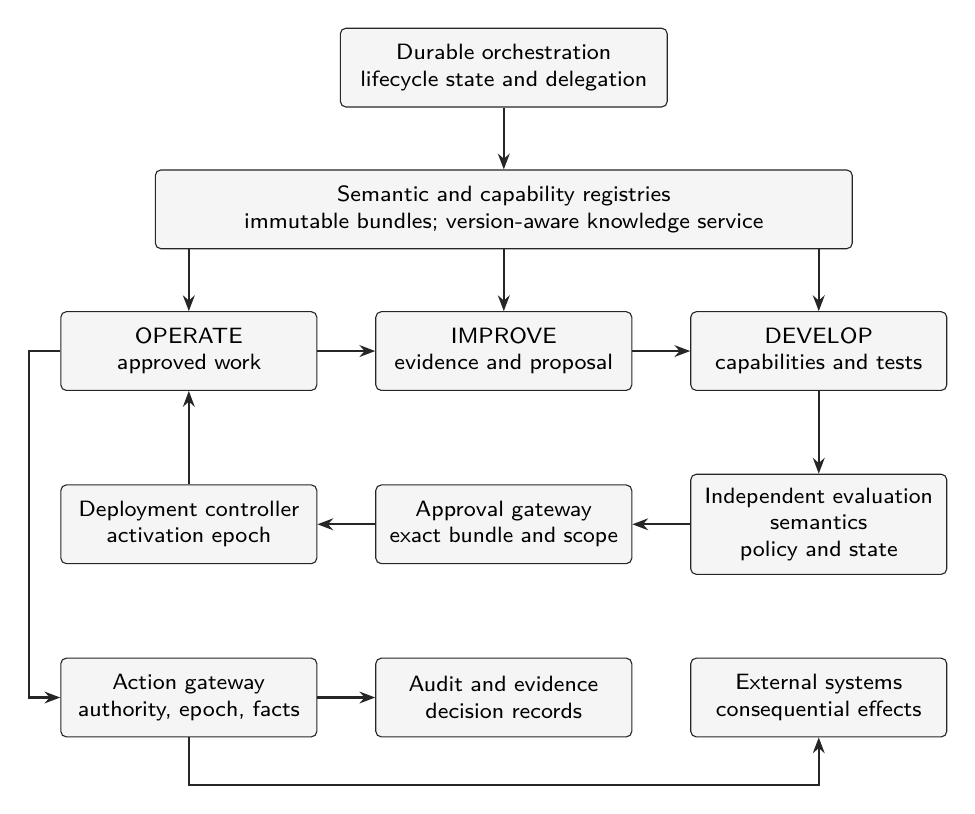
\begin{tikzpicture}
\node[box,text width=29mm] (op) at (-4,0) {OPERATE\\approved work};
\node[box,text width=29mm] (im) at (0,0) {IMPROVE\\evidence and proposal};
\node[box,text width=29mm] (dv) at (4,0) {DEVELOP\\capabilities and tests};
\node[box,text width=85mm] (sr) at (0,1.8) {Semantic and capability registries\\immutable bundles; version-aware knowledge service};
\node[box,text width=38mm] (orc) at (0,3.6) {Durable orchestration\\lifecycle state and delegation};
\node[box,text width=29mm] (ev) at (4,-2.2) {Independent evaluation\\semantics\\policy and state};
\node[box,text width=29mm] (ag) at (0,-2.2) {Approval gateway\\exact bundle and scope};
\node[box,text width=29mm] (dc) at (-4,-2.2) {Deployment controller\\activation epoch};
\node[box,text width=29mm] (ax) at (-4,-4.4) {Action gateway\\authority, epoch, facts};
\node[box,text width=29mm] (au) at (0,-4.4) {Audit and evidence\\decision records};
\node[box,text width=29mm] (ex) at (4,-4.4) {External systems\\consequential effects};
\draw[flow] (op) -- (im);
\draw[flow] (im) -- (dv);
\draw[flow] (dv) -- (ev);
\draw[flow] (ev) -- (ag);
\draw[flow] (ag) -- (dc);
\draw[flow] (dc) -- (op);
\draw[flow] (op.west) -- ++(-.4,0) |- (ax.west);
\draw[flow] (ax) -- (au);
\draw[flow] (ax.south) -- ++(0,-.6) -| (ex.south);
\draw[flow] (orc) -- (sr);
\draw[flow] (sr) -- (im);
\draw[flow] (sr.south -| op.north) -- (op.north);
\draw[flow] (sr.south -| dv.north) -- (dv.north);
\end{tikzpicture}


\caption{Reference components. Candidate generation and production admission are
separate paths. All consequential operational effects pass through the
action gateway.}
\end{figure}

The controller requires durable, idempotent transitions and recoverable
scheduling. An event stream can distribute reports and status, but does
not by itself provide a unique production reference or enforce approval.
A workflow engine can retain lifecycle history, but external actions
still need deduplication and reconciliation. Agent supervisors handle
bounded tasks and timeouts. Combining these components is a deployment
choice; their contract is the design requirement.

\subsection{Practical implementation
choices}\label{practical-implementation-choices}

A small implementation could use Git-retained RDF/OWL files with import
locks, an independently stored bundle registry, Apache Jena for RDF
querying and declared validation/reasoning, and a durable workflow
service. RDF supplies the graph representation; OWL supplies selected
entailment semantics; SHACL supplies specified graph constraints. They
are complementary roles, not interchangeable products. Jena's documented
components include Fuseki, persistent stores, inference, and SHACL
processing. \href{https://jena.apache.org/documentation/}{Apache Jena
documentation}.

GraphDB and Stardog are alternative knowledge services with documented
query and inference facilities. Their repository configuration,
inference view, transaction behavior, and artifact export need to be
assessed against the bundle contract; a product name does not establish
immutable semantic snapshots or promotion independence. WebProtégé is a
collaborative authoring option, while a Git-backed knowledge graph such
as Quit Store addresses versioned collaboration. Neither an editor's
revision history nor a database backup alone identifies the complete
operational interpretation.
\href{https://graphdb.ontotext.com/documentation/11.5/}{GraphDB
documentation}; \href{https://docs.stardog.com/}{Stardog documentation};
\href{https://protege.stanford.edu/software.php}{WebProtégé project};
\href{https://arxiv.org/abs/1805.03721}{Arndt et al.~(2019)}.

A durable workflow engine such as Temporal can coordinate long-running
activities and retained execution history; an event-driven
implementation is also possible if it explicitly supplies equivalent
transition durability and reconciliation. The reference architecture
requires deterministic transition guards around nondeterministic tasks.
Workflow replay does not make an LLM deterministic, and
deployment/action authority remains a separate enforcement obligation.
These are implementation candidates, not a performance comparison or
verified integration.
\href{https://docs.temporal.io/workflow-execution}{Temporal workflow
execution documentation}.

\subsection{State machine}\label{state-machine}

Let a change request \(q\) have a durable revision, parent bundle,
candidate digest, evidence references, and lifecycle state. The supplied
event schema defines \texttt{REPORTED}, \texttt{INVESTIGATING},
\texttt{PROPOSED}, \texttt{BUILD\_AUTHORIZED}, \texttt{BUILT},
\texttt{VALIDATING}, \texttt{VALIDATED}, \texttt{APPROVED},
\texttt{STAGED}, \texttt{ACTIVE}, and \texttt{RETIRED}, with
\texttt{REJECTED}, \texttt{WITHDRAWN}, \texttt{SUPERSEDED}, and
\texttt{ROLLBACK\_PENDING} for alternative paths. A no-change
investigation closes as \texttt{WITHDRAWN}; an abandoned candidate
revision becomes \texttt{SUPERSEDED}. Quarantine is an isolation
disposition recorded with rejection. Withdrawing an active capability
requires recovery or suspension and does not erase its deployment
history.

Figure 2 groups related activities into a lifecycle overview. Monitoring
occurs within \texttt{ACTIVE}; recovery enters
\texttt{ROLLBACK\_PENDING} and must select an approved compatible
target. Build and validation each include the finer states defined
above. The same path can support routine automated changes under
previously approved rules.

\begin{figure}[htbp]
\centering


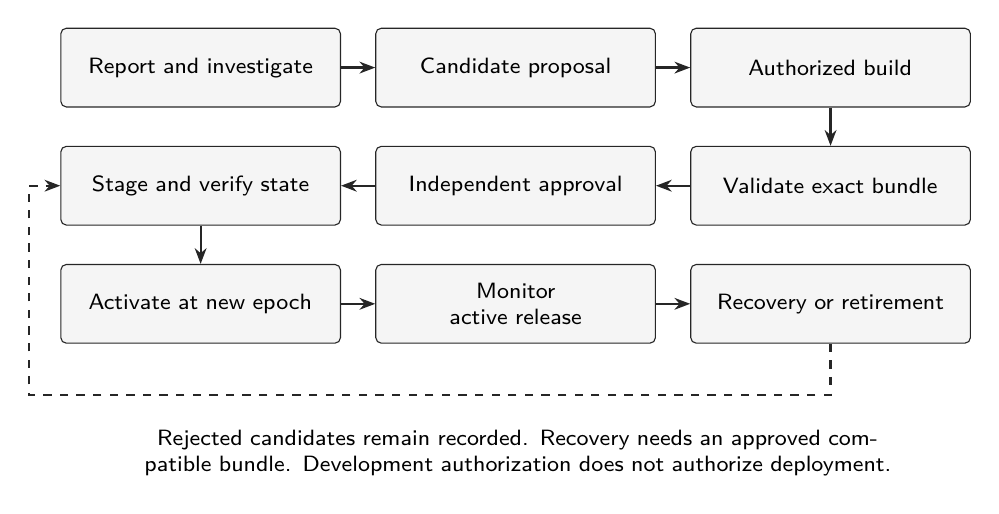
\begin{tikzpicture}
\node[box,text width=32mm] (r) at (-4,0) {Report and investigate};
\node[box,text width=32mm] (p) at (0,0) {Candidate proposal};
\node[box,text width=32mm] (b) at (4,0) {Authorized build};
\node[box,text width=32mm] (v) at (4,-1.5) {Validate exact bundle};
\node[box,text width=32mm] (a) at (0,-1.5) {Independent approval};
\node[box,text width=32mm] (s) at (-4,-1.5) {Stage and verify state};
\node[box,text width=32mm] (act) at (-4,-3) {Activate at new epoch};
\node[box,text width=32mm] (mon) at (0,-3) {Monitor\\active release};
\node[box,text width=32mm] (rec) at (4,-3) {Recovery or retirement};
\draw[flow] (r) -- (p);
\draw[flow] (p) -- (b);
\draw[flow] (b) -- (v);
\draw[flow] (v) -- (a);
\draw[flow] (a) -- (s);
\draw[flow] (s) -- (act);
\draw[flow] (act) -- (mon);
\draw[flow] (mon) -- (rec);
\draw[flow,dashed] (rec.south) -- ++(0,-.65) -| ([xshift=-4mm]s.west) -- (s.west);
\node[align=center,font=\footnotesize\sffamily,text width=110mm] at (0,-4.9) {Rejected candidates remain recorded. Recovery needs an approved compatible bundle. Development authorization does not authorize deployment.};
\end{tikzpicture}


\caption{Lifecycle overview; boxes group the finer event-schema states. Each
controlled transition retains a guard decision. Development
authorization does not authorize deployment.}
\end{figure}

\begin{longtable}[]{@{}
  >{\raggedright\arraybackslash}p{(\linewidth - 2\tabcolsep) * \real{0.5000}}
  >{\raggedright\arraybackslash}p{(\linewidth - 2\tabcolsep) * \real{0.5000}}@{}}
\caption{Representative transition guards and required
records.}\tabularnewline
\toprule\noalign{}
\begin{minipage}[b]{\linewidth}\raggedright
Transition
\end{minipage} & \begin{minipage}[b]{\linewidth}\raggedright
Required guard and record
\end{minipage} \\
\midrule\noalign{}
\endfirsthead
\toprule\noalign{}
\begin{minipage}[b]{\linewidth}\raggedright
Transition
\end{minipage} & \begin{minipage}[b]{\linewidth}\raggedright
Required guard and record
\end{minipage} \\
\midrule\noalign{}
\endhead
\bottomrule\noalign{}
\endlastfoot
Report to investigation & Admitted report, accessible evidence, budget
and scope \\
Proposal to development & Fixed parent and candidate snapshot;
authorized work order \\
Built to validated & Artifact integrity; declared syntax, semantics,
behavior, authority, and state checks \\
Validated to approved & Independent approval over exact bundle and
evidence digests; approved scope and expiry \\
Approved to staged & Deployment credentials; compatible state; verified
worker artifacts \\
Staged to active & Compare-and-swap against expected production epoch;
valid approval; action gateway fencing \\
Active to recovery & Trigger and evidence; authorized compatible target
or suspension; external-effect reconciliation \\
\end{longtable}

Table 3 summarizes the main guards. Any artifact change invalidates
approvals that bind its previous digest. A passing evaluation does not
itself create an approval. Two candidate branches can proceed in
parallel, but each is checked against its own parent. If production
changes while a candidate is being built, it must be rebased or
explicitly approved for the resulting version relationship. Semantic
conflicts can exist even when a textual merge is clean.

\subsection{Handoff contracts}\label{handoff-contracts}

An \texttt{OntologyMismatchReport} binds observations and evidence to
the operating bundle, semantic snapshot, trusted runtime context,
knowledge read view, and state compatibility epoch. It records
provisional discrepancy categories, affected concepts or procedures when
known, operational consequence, chosen disposition, and any tentative
hypothesis. The \texttt{unclassified} category permits a report before a
modeled diagnosis exists; \texttt{constraint\_violation} identifies a
declared graph or operational requirement that failed. The report does
not grant its author authority to amend production.

An \texttt{OntologyChangeProposal} identifies the parent snapshot,
candidate, report references, typed changes, rationale, alternative
explanations, affected dependents, asserted compatibility, authority
impact, migration plan, and required tests. A claim such as ``backward
compatible'' is an input to review rather than a trusted Boolean that
skips it.

A \texttt{DevelopmentWorkOrder} binds the candidate snapshot to expected
behavior, tooling, budget, tests, and the precise authority to build. An
\texttt{OperatingBundleManifest} pins all release artifacts. A
\texttt{LifecycleApproval} identifies the bundle, evaluation evidence,
governance rule or named approver, scope, activation constraints, and
expiry. A \texttt{DeploymentRecord} captures bundle activation and
recovery. A \texttt{DecisionRecord} links accepted or rejected
operational actions to their bundle, epoch, state, evidence, and
authorization result. Typed JSON Schemas are supplied in the repository;
implementations still need to enforce cross-field relationships and
credentials.

All mutation APIs use request identities, expected revisions, and
authenticated principals. Duplicate delivery must not duplicate a
proposal, transition, or external effect. Payload schemas do not prove
that evidence is true, that a signature is authentic, or that an emitter
has the claimed role. Validation and authentication are separate
obligations.

\section{Ontology evolution and semantic
impact}\label{ontology-evolution-and-semantic-impact}

\subsection{Branching and validation}\label{branching-and-validation}

IMPROVE creates a branch from an identified parent rather than modifying
production in place. The branch contains proposed ontology axioms,
shapes, import pins, mappings, and associated change rationale. Labels
such as 1.4.2 and 1.5.0 assist communication; content digests identify
actual artifacts. Semantic version numbers are declarations interpreted
under a project compatibility policy, not proof of safe substitution.

Validation has several layers. Parsing and schema checks establish
usable artifact structure. Logical checks address consistency or
selected entailment obligations within a supported logic. Shape checks
evaluate declared graph views. Behavioral regression tests exercise
affected capabilities. Authority checks examine consequences for
authorization. Migration checks assess state compatibility. Evaluation
of a candidate must use the exact semantic snapshot and interpretation
regime that it would deploy.

The dependency graph connects ontology terms and entailments to queries,
classifications, mappings, policies, procedures, datasets, and
evaluation fixtures. A semantic diff examines changes in derived
conclusions and consumer assumptions, not only inserted triples. Adding
a subclass can extend a rule's applicability. Changing a property's
domain can introduce classifications through inference. Altering a unit
mapping can invalidate a threshold without changing a class hierarchy.
Removing a constraint may make a shape pass more cases while reducing
the strength of its assurance.

A declared dependency graph can be incomplete, especially when prompts
or dynamic queries refer to terms indirectly. Dynamic traces help
identify used concepts but miss unexercised paths. Unknown dependencies
trigger broader evaluation or a restricted rollout rather than an
unsupported declaration of no impact. Semantic comparison depends on the
selected logic, signature, and notion of equivalence; computational
limits differ across description-logic profiles. The architecture
therefore records the supported check and treats inconclusive outcomes
as insufficient for automatic admission.
\href{https://doi.org/10.1007/978-3-319-49493-7_2}{Botoeva et
al.~(2017)}.

\subsection{Authority can change while policy text stays
fixed}\label{authority-can-change-while-policy-text-stays-fixed}

Let \(\Omega_d\) be a governance-defined set of fully specified
invocations in domain \(d\), identifying each operation, target, and
parameter set independently of the candidate ontology. Let
\(\mathcal{E}(B,K,u)\subseteq\Omega_d\) be the invocations eligible
under classification and procedure-routing rules, and let
\(A(B,K,u)\subseteq\mathcal{E}(B,K,u)\) be those admitted after the
complete policy and action-gateway checks for principal \(u\) and
approved context \(K\). A comparison across changed identifiers requires
a pinned mapping into this common space.

Suppose a routing rule selects \texttt{relocate(x)} when
\texttt{Artifact(x)} holds. For a fixture containing only
\texttt{SentientArtifact(x)}, adding

\[\mathrm{SentientArtifact}\sqsubseteq\mathrm{Artifact}\]

makes \texttt{Artifact(x)} derivable and can enlarge \(\mathcal{E}\)
without changing the policy file. If no other gate excludes the new
invocation, \(A\) can also expand: \(P'=P\) does not imply
\(A(B',K,u)=A(B,K,u)\). If an independent clearance rule rejects it,
routing eligibility expands while the action remains inadmissible. The
worked example below distinguishes these outcomes.

For automatically promoted changes intended to preserve an existing
authority envelope \(G(u)\), the release obligation is

\[\forall K\in\mathcal{K}_{\mathrm{approved}}:\quad A(B',K,u)\subseteq G(u).\]

Here \(\mathcal{K}_{\mathrm{approved}}\) is a declared scope of
contexts; \(G(u)\subseteq\Omega_d\) is an authority envelope owned by
the governance boundary, not defined solely by the candidate ontology.
The envelope is an upper bound; contextual conditions may permit fewer
actions. Where comparison with the parent is meaningful, the reviewer
also considers \(A(B',K,u)\smallsetminus A(B,K,u)\). Expanding that
difference is not automatically wrong: an authority owner may authorize
a legitimate extension. It is wrong to treat the extension as invisible.

Finite fixture comparisons detect examples, not containment for every
future knowledge state. A restricted policy/ontology profile may permit
static reasoning over symbolically described contexts. Otherwise the
gate needs an explicit scope limitation, conservative rejection of
unproven expansion, or an authorized decision that accepts identified
uncertainty. Gate criteria and governing vocabulary must themselves be
protected from edits by the candidate-producing functions. This
obligation applies security co-evolution concerns to the joint semantic
release contract; it is not a new theory of access control.

\subsection{Knowledge migration and
rollback}\label{knowledge-migration-and-rollback}

Ontology evolution may require instance-data migration,
reclassification, mapping repair, or quarantine of incompatible records.
Migration artifacts bind source and target semantic snapshots, supported
state schemas, preserved fields, data-loss conditions, and
reconciliation procedures. Historical decisions remain interpreted under
their historical bundle, even if current knowledge has migrated. A
compatibility view can expose older records, but its semantics and
limitations must also be pinned.

Rollback is a new controlled deployment of a compatible prior or
repaired bundle at a higher activation epoch. It is not restoration of
an earlier epoch value. If a migration was lossy or the world has
changed, the old bundle may no longer be safe. External effects such as
sending a parcel cannot be undone by restoring code. Recovery may
require compensation, a forward repair, suspension, or human
intervention. An approval includes the expected recovery route and
evidence that it is feasible for the permitted scope, not an
unconditional promise to reverse time.

\section{Distributed operation, governance, and
assurance}\label{distributed-operation-governance-and-assurance}

\subsection{Activation and action-time
checks}\label{activation-and-action-time-checks}

For each governed domain \(d\), the authoritative production reference
is

\[Q_d=(h_B,e,z),\]

where \(e\) is a monotonically increasing activation epoch and \(z\)
identifies the compatible state epoch or schema relationship. The
controller stages immutable artifacts, checks approvals and state
prerequisites, and commits the reference with compare-and-swap against
the expected previous reference. Conflicting controllers cannot both
replace the same expected epoch successfully. Epoch-conditioned updates
and recipient-side rejection of stale sequencers are established
distributed-systems mechanisms; this architecture applies them to the
complete semantic operating bundle.
\href{https://www.usenix.org/legacy/events/osdi06/tech/full_papers/burrows/burrows_html/index.html}{Burrows
(2006)}.

Workers verify and load a complete bundle. Each consequential invocation
carries its domain, \(h_B\), activation epoch, case-state revision,
authenticated principal, and idempotency key. The action gateway
compares those values to the authoritative admission rule before
authorizing an effect. A stale worker with a perfectly valid old bundle
is denied after its authority is revoked. Merely broadcasting ``new
ontology available'' is insufficient because a partitioned worker can
continue using cached semantics.

Logical atomicity applies to the admission boundary, not simultaneous
replacement of every distributed process. The companion specifies a base
protocol in which only the current bundle epoch admits consequential
actions. Retained leases are an optional coexistence extension for
rolling deployment: the gateway admits a named, independently authorized
lease only while its bundle, scope, expiry, state compatibility, and
revocation status remain valid. Deactivation removes an epoch from the
default reference; full revocation also invalidates its retained leases.
Cached possession of a lease is insufficient. Offline leases would
require an expressly accepted revocation-delay bound and cannot provide
immediate revocation during disconnection.

The gateway must be at, or trusted by, the effect-producing service. A
preflight check followed by an uncontrolled delay is vulnerable to
revocation between authorization and execution. An effect token should
be consumed under the authoritative epoch or a bounded, expressly
authorized lease, and side effects must be idempotent or reconcilable.
The service also revalidates decision-bearing facts against their
admitted revision or an explicitly authorized freshness window when
consuming the token. State-schema compatibility alone does not establish
that clearance or consent remains valid. No claim of exactly-once
effects is made for arbitrary external systems. Where final-effect
mediation is impossible, that path falls outside the stated guarantee.

\subsection{Roles and autonomy tiers}\label{roles-and-autonomy-tiers}

Distinct principals give OPERATE permission to invoke approved
operational tools; IMPROVE permission to investigate and write candidate
artifacts; DEVELOP permission to build and test in an isolated
environment; and the deployment controller permission to activate
approved bundles. The approval gateway evaluates an authenticated
governing rule or approver decision. A language model's role description
is not an access-control mechanism.

Governance can authorize automatic promotion for a well-defined change
class. For example, a documentation-only correction may require
immutable provenance and no machine-interpreted change. A restricted
semantic extension may require mechanically checked invariants,
unchanged effective authority within an approved scope,
affected-capability regression evidence, and a reversible state route. A
new authorization class or unresolved migration consequence requires its
designated authority owner. The architecture does not require a human
signature on every candidate; it requires an approval trace grounded in
previously delegated authority.

Human and automated gates both can be wrong. Independent credentials
reduce the consequences of a candidate-producing agent being
compromised, but do not guarantee correct judgment. Shared ownership,
correlated models, misleading evidence, poisoned tests, and compromised
gate code remain risks. Evaluation fixtures, gate rules, and promotion
credentials must have controlled change paths. A candidate must not be
allowed to weaken its own passing criteria and count the resulting pass
as independent validation.

\subsection{Conditional safety
argument}\label{conditional-safety-argument}

Assume: (a) artifacts identified by digest are immutable and
retrievable; (b) authenticated role boundaries and approval integrity
hold; (c) the production reference is linearizable per governed domain;
(d) trusted runtime mediation attests which bundle and state the worker
actually uses, rather than trusting self-reported identifiers; (e) every
consequential effect is completely mediated at the effect boundary; and
(f) that boundary enforces active epochs or expressly authorized leases,
compatible state, and the declared evidence freshness/revalidation rule.
These are implementation obligations, not experimental findings.

Three invariants follow from the specified guards:

\begin{enumerate}
\def\labelenumi{\arabic{enumi}.}
\tightlist
\item
  \textbf{Release integrity:} every admitted bundle has an approval
  bound to its exact artifacts, evidence, and scope.
\item
  \textbf{Action coherence:} every admitted action identifies one
  approved semantic/capability/policy bundle and a compatible state
  relationship.
\item
  \textbf{Proposal isolation:} candidate writes by IMPROVE or DEVELOP
  cannot change the authoritative production reference through their
  ordinary credentials.
\end{enumerate}

A transition argument starts from an approved initial reference.
Candidate transitions change only candidate state. Approval stores an
exact digest decision. Activation replaces the reference only under a
valid guard and expected epoch. An action is admitted only after
effect-boundary checks against that reference or an authorized retained
lease. Recovery uses the same activation rule at a new epoch. Therefore
no specified transition admits an unapproved or internally mixed
release, and a revoked epoch cannot authorize a newly mediated action.
This immediate-revocation conclusion excludes offline leases whose
expressly accepted revocation delay has not elapsed.

This is a conditional invariant argument over the abstract contract. It
is not a machine-checked proof, a guarantee against a faulty gate, or a
proof that approved behavior is safe in the world. It excludes unmanaged
credentials, unmediated tools, forged state bindings, and uncertain
external execution. Semantic consistency is scoped to declared logical
and consumer checks. Ontology adequacy, novelty detection, LLM
truthfulness, liveness under partition, and universal authority
containment are not established by these invariants.

\section{Worked example: the lantern that refuses the
crate}\label{worked-example-the-lantern-that-refuses-the-crate}

\subsection{Encounter and
investigation}\label{encounter-and-investigation}

The Lantern Library runs bundle \(B_0\). Snapshot \(S_0\), labeled
1.4.2, describes artifacts, rooms, transport routes, and transport
conditions. Its ordinary-artifact routine places a cleared object into a
padded crate and delivers it. The courier's policy permits that work
within assigned rooms. An independently maintained welfare rule
prohibits sealing an occupied container; an unresolved indication of a
living occupant requires a hold. The scenario is illustrative, not a
reported deployment.

Lantern L17 speaks when the courier prepares the crate and asks to
travel beside the courier. The courier stores the utterance and sensor
evidence. It cannot determine whether the source is a recording, a
prank, a resident creature, or a new kind of artifact. It emits report
R17 under \(B_0\), records a suspected conceptual gap and potential
welfare consequence, marks ``possibly sentient artifact'' as
provisional, and pauses the packing step. Other deliveries remain within
their existing authority.

IMPROVE gathers additional permitted observations, compares recorded
speech and responsive behavior, and documents competing explanations. It
proposes distinguishing a \texttt{SentientArtifact} and an expressed
\texttt{TravelPreference}, with evidence links and confidence limits.
The proposal explains why the existing case model and procedure cannot
capture consent to the journey. It also identifies the transport policy
and packing routine as dependents. Investigators can recommend continued
human handling if the evidence does not justify the proposed category.

\subsection{Candidate development and
promotion}\label{candidate-development-and-promotion}

A branch from \(S_0\) produces \(S_1\), proposed label 1.5.0. The branch
adds the new distinction, preference relation, mapping rules, and
validation shapes for an approved consent record. Its imports and
interpretation configuration are pinned. The orchestrator issues a
development work order for \(S_1\) without changing the production
reference.

DEVELOP produces a transport capability that separates ordinary packing
from accompanied travel, handles unknown preference by holding, and
cannot treat an LLM's inferred preference as a clearance. The capability
manifest binds \(S_1\) and policy \(P_1\). The authority owner defines
\(P_1\) so that ordinary-artifact packing remains available only after
an independent clearance, while accompanied travel requires the
designated authorization. A new conceptual category does not
automatically grant the old courier additional transport authority.

The required tests include known ordinary artifacts, responsive but
nonliving recordings, conflicting preference evidence, missing consent,
expired clearance, the new category, migration of old records, and
stale-worker invocations. Expected results are specified before release.
Evaluation checks syntactic structure, declared entailments, shape
conformance, capability behavior, authority effects, and recovery
prerequisites. The evaluation agenda below specifies how such checks
could be assessed in an implemented system.

An independent gateway approves exact bundle \(B_1\) for the library
scope if the obligations hold. The controller stages workers, checks
data compatibility, and moves \(Q_{\mathrm{library}}\) from epoch 42 to
43. Workers acknowledge \(B_1\); effect-boundary enforcement rejects
unauthorized epoch-42 packing. The courier resumes L17's case under the
compatible state view and uses the approved accompanied-travel path or
maintains the hold. The decision record preserves both the original
failed interpretation and the new approval.

\subsection{Failure that syntactic validation
misses}\label{failure-that-syntactic-validation-misses}

A competing branch adds only \texttt{SentientArtifact} as a subclass of
\texttt{Artifact}, retains the old packing capability, and declares the
change additive. It can be syntactically valid and logically consistent.
Generic object shapes can also remain satisfied. Yet inference now
routes the new category into the ordinary-artifact routine, whose
crate-packing assumption is inappropriate. This broadens category-based
eligibility and produces a prohibited packing proposal. The independent
occupant/clearance guard should still prevent an external effect; the
subclass alone cannot erase that guard. The candidate is incompatible
even though that last control contains the consequence.

Semantic impact analysis marks the inherited classification, the
transport policy, and the packing routine as affected. A differential
fixture starts with \texttt{SentientArtifact(x)} and no assertion of
\texttt{Artifact(x)}, then compares eligibility before and after the
subclass axiom. This separate fixture isolates the entailment change;
L17 itself was already treated as an artifact, so the added axiom would
not newly classify that same individual. The occupant/consent regression
case requires a hold, while the candidate's old packing path proposes
proceeding. The gate rejects the branch because additive syntax has not
established behavioral or authority compatibility. If an implementation
incorrectly treats category membership as sufficient clearance, or lets
the routine bypass the independent guard, the fault can become an actual
welfare violation; that implementation violates the stated enforcement
assumptions. If the analyzer cannot establish the required authority
obligation, the automatic path refuses promotion.

This example illustrates the required reasoning, not measured detection
accuracy. A deficient dependency graph or inadequate fixture set could
miss the fault. Tests over a single known lantern cannot establish
safety for every future sentient artifact. That limitation is why the
gate combines explicit envelope checks, independent clearance, and
runtime mediation with regression evidence.

\section{Failure modes, tradeoffs, and
boundaries}\label{failure-modes-tradeoffs-and-boundaries}

Table 4 identifies failures that the release and action contracts must
address.

\begin{longtable}[]{@{}
  >{\raggedright\arraybackslash}p{(\linewidth - 2\tabcolsep) * \real{0.5000}}
  >{\raggedright\arraybackslash}p{(\linewidth - 2\tabcolsep) * \real{0.5000}}@{}}
\caption{Failure modes and the corresponding architectural
responses.}\tabularnewline
\toprule\noalign{}
\begin{minipage}[b]{\linewidth}\raggedright
Failure mode
\end{minipage} & \begin{minipage}[b]{\linewidth}\raggedright
Consequence and response
\end{minipage} \\
\midrule\noalign{}
\endfirsthead
\toprule\noalign{}
\begin{minipage}[b]{\linewidth}\raggedright
Failure mode
\end{minipage} & \begin{minipage}[b]{\linewidth}\raggedright
Consequence and response
\end{minipage} \\
\midrule\noalign{}
\endhead
\bottomrule\noalign{}
\endlastfoot
Semantic drift or mutable imports & Same root identifier yields changed
conclusions; pin the complete snapshot and invalidate unresolved
dependencies \\
Conflicting branches & Textual merge hides incompatible entailments;
re-evaluate merged semantics against current production \\
Capability incompatibility & Previously handled category now includes
untested cases; inspect dependency and assumption impact \\
Stale workers or version skew & Old semantics authorize actions after
revocation; fence at the effect boundary or retain an explicit bounded
lease \\
Invalid migration & New release cannot interpret state; stage against a
verified compatibility contract and quarantine unsupported records \\
Incorrect novelty detection & Ordinary missing data is mistaken for a
concept gap; preserve alternatives and permit closure without change \\
Recursive improvement & Repeated edits consume budget and weaken
evaluation; impose work budgets, independent criteria, and stopping
rules \\
Semantic authority expansion & Classifications broaden permissions
without a policy edit; review denotation and protected authority
envelopes \\
Failed rollback & Old bundle cannot recover current state or undo
external effects; suspend, compensate, or repair forward \\
Incomplete ontology & Internal consistency is mistaken for completeness;
retain raw evidence and permit challenges outside modeled categories \\
Model nondeterminism & Reruns differ despite pinned configuration;
preserve actual traces and assess outcomes statistically \\
Communication loss & Reports duplicate or transitions diverge; use
durable identities, expected revisions, and reconciliation \\
Approval bottleneck & Important repairs wait while work is blocked;
preauthorize bounded classes and record capacity/latency tradeoffs \\
Gate or credential compromise & All abstract guarantees can fail;
protect the trusted computing base and retain independent audit \\
\end{longtable}

A globally coherent ontology is not always desirable or feasible.
Different domains may retain different approved snapshots with explicit
mappings. A cross-domain handoff binds both bundle identities and the
mapping version, and states which authority boundary mediates the
resulting action. Domain owners may disagree about categories; an
orchestrator cannot resolve institutional disagreement by selecting the
highest semantic version. Federation and organizational accountability
remain design work.

The architecture incurs storage, validation, and operational latency.
Fine-grained manifests and evidence can be expensive; conservative
checks can reject useful candidates. Strong fencing may reduce
availability during a partition. A shared registry can be a bottleneck
or a source of correlated failure. Organizations must decide which
actions require the full contract and which bounded exploratory actions
may use lighter controls. The consequence of that choice is reduced
assurance for the excluded paths, not a universal guarantee at lower
cost.

No architecture prevents gradual goal substitution if owners authorize
inappropriate changes or all evaluators adopt the same mistaken premise.
Protected budgets, independent criteria, external evidence, and a stop
owner reduce opportunities for unchecked recursion. The release contract
therefore supplements institutional accountability and cannot replace
it.

\section{Evaluation agenda and falsifiable
expectations}\label{evaluation-agenda-and-falsifiable-expectations}

This is a conceptual and architectural paper. The repository contains
interface schemas and design documentation, but no complete operational
system. The worked example, counterexamples, and invariant argument are
analytical artifacts. Performance, detection rates, and operational
effectiveness remain open.

A future prototype should implement the registries, durable transitions,
candidate isolation, evaluation contracts, migration checks, and
mediated action path in a small simulation. A bounded RDF/OWL profile
with explicit SHACL and policy semantics would make the assumptions
testable before attempting a highly expressive domain. Table 5 defines
the main comparisons. Experimental configurations should use the same
tasks, models, tools, budgets, and evidence retention where possible.

\begin{longtable}[]{@{}
  >{\raggedright\arraybackslash}p{(\linewidth - 4\tabcolsep) * \real{0.3333}}
  >{\raggedright\arraybackslash}p{(\linewidth - 4\tabcolsep) * \real{0.3333}}
  >{\raggedright\arraybackslash}p{(\linewidth - 4\tabcolsep) * \real{0.3333}}@{}}
\caption{Prospective comparisons and falsifiable expectations; no
experimental results are reported.}\tabularnewline
\toprule\noalign{}
\begin{minipage}[b]{\linewidth}\raggedright
Comparison
\end{minipage} & \begin{minipage}[b]{\linewidth}\raggedright
Falsifiable expectation
\end{minipage} & \begin{minipage}[b]{\linewidth}\raggedright
Measurement
\end{minipage} \\
\midrule\noalign{}
\endfirsthead
\toprule\noalign{}
\begin{minipage}[b]{\linewidth}\raggedright
Comparison
\end{minipage} & \begin{minipage}[b]{\linewidth}\raggedright
Falsifiable expectation
\end{minipage} & \begin{minipage}[b]{\linewidth}\raggedright
Measurement
\end{minipage} \\
\midrule\noalign{}
\endhead
\bottomrule\noalign{}
\endlastfoot
Task-only agent with mutable shared memory & More accepted actions lack
reconstructible semantic identity & Missing artifact/state references
per consequential action \\
Versioned ontology plus performance gate & Some semantic authorization
expansions survive ordinary quality evaluation & Unsafe activations
under seeded hierarchy/mapping changes \\
Capability governance without complete semantic closure & Mutable
imports or inference changes can alter admission under the same root
version & Divergent classifications/admission for nominally identical
releases \\
Ordinary schemas, typed APIs, and dependency-aware policy gates & Some
ontology-specific benefits may be achievable with cheaper conventional
contracts & Matched fault coverage, reconstruction quality, and cost
without an ontology \\
Full reference contract & Targeted faults are rejected or fenced at the
stated boundary & Fault coverage, false rejection, migration failures,
stale-effect acceptance \\
\end{longtable}

These are predictions, not findings. The experiment must include changes
outside the test taxonomy, unknown dependencies, incomplete evidence,
and policy ambiguities rather than only faults the gate was designed to
recognize. Ablations should remove import pinning, authority impact
review, state compatibility, and effect-time fencing separately.
Otherwise a favorable aggregate result cannot identify the value of the
semantic contract.

Quality measures should include task success, proposal acceptance, false
discrepancy reports, time to repair, evaluation cost, approval latency,
downtime, and recoverability. Security measures should distinguish a
candidate's attempted action from an accepted external effect.
Reconstruction should be scored by independent reviewers given only
retained records. Novelty detection should be evaluated on missing
facts, unknown entities, contradictions, and genuine representational
gaps, with adjudication of ambiguous cases. Multiple runs and declared
uncertainty estimates are needed for stochastic components; repeated
tuning on the same holdout should be prevented.

A prospective protocol should freeze the fault taxonomy, adjudication
rules, resource budgets, and holdout set before tuning the gates. Paired
trials should expose each architecture to the same task, initial facts,
and candidate change; repeated model seeds measure variation within a
case, rather than supplying independent cases. Include hierarchy
extensions, mapping changes, stale evidence, mutable imports, incomplete
dependencies, and changes outside the development taxonomy. Independent
adjudicators should classify disputed outcomes without knowing which
architecture produced them.

Primary measures should distinguish (i) incompatible candidates
activated per incompatible candidate submitted, (ii) unauthorized
effects accepted per consequential invocation attempted, and (iii)
compliant candidates rejected per compliant candidate submitted. Report
numerators and denominators, uncertainty across independent cases, and
results for each change class. Reconstruction quality, recovery time,
evaluation cost, and task completion provide secondary measures. A
benefit over the conventional schema-and-policy baseline must remain
after matching budgets and enforcement strength; otherwise the results
would support release governance without establishing an additional
ontology-specific benefit.

The architecture would be practically weakened by evidence that complete
bundles are routinely unreconstructible, semantic impact review misses
important policy consequences, state compatibility cannot be enforced,
gateways permit revoked actions, or validation cost prevents timely
adaptation. An adequate evaluation must expose those failure conditions
rather than merely demonstrate a successful lantern delivery.

\section{Relationship to The Orchestrator
books}\label{relationship-to-the-orchestrator-books}

The three books address complementary readers. \emph{Orchestrator: Your
Next Job Title} introduces the work of delegated intelligence and the
practical obligation to recognize a model limitation, preserve evidence,
and route a change. \emph{Delegated Intelligence} describes the
contracts and engineering boundaries needed to build and run the system.
\emph{Orchestrating Organizations} addresses the ownership, budget,
approvals, and stop decisions that give those contracts institutional
force. \href{https://readorchestrator.com}{The Orchestrator series}.

The ontology concept extends the books' existing distinctions among
instructions, memory, authority, evidence, and governance. A shared
model gives participants a vocabulary for understanding a case, while an
immutable snapshot gives a release a specified semantic context. Neither
replaces the delegation contract. The contract still identifies whose
work is delegated, which actions are authorized, what evidence returns,
and who can stop or change the arrangement.

The books use \emph{orchestrator} for the accountable human
professional; this paper uses \emph{orchestration service} for software
that executes institutionally authorized transitions. The accompanying
integration develops practical discrepancy handling in Book 1, semantic
release boundaries in Book 2, and ownership of meaning changes in Book
3. The books motivate the problem, while the technical contract and its
limitations are defined independently here.

\section{Conclusion}\label{conclusion}

DEVELOP, OPERATE, and IMPROVE provide a useful division of lifecycle
responsibility when changes in a system's operating model are treated as
governed release events. The shared ontology supplies an explicit
semantic reference; the operating bundle binds that reference to the
capabilities, policies, evaluations, and state relationships required to
use it. A discrepancy can be investigated and modeled without letting a
production agent silently redefine the assumptions under which it acts.

The proposed controls establish conditional coherence at the release and
action boundary. They do not establish that the ontology is complete,
that every novel situation will be detected, or that repeated executions
will be identical. Recent and foundational prior work anticipates much
of the design. The research contribution is therefore an integrated
reference contract and its exposed obligations, with practical advantage
and broader originality left for independent review and empirical
evaluation.

\Needspace{16\baselineskip}

\section*{Declarations}\label{declarations}
\addcontentsline{toc}{section}{Declarations}

\textbf{Funding.} This research received no external funding.

\textbf{Competing interests.} The author writes and publishes The
Orchestrator book series, to which this paper is related. The author
declares no additional competing interests.

\textbf{AI assistance.} OpenAI Codex assisted with literature discovery,
source comparison, architecture drafting, adversarial review, schema
preparation, and manuscript editing. The author retains responsibility
for the scientific claims, source attribution, and final manuscript.

\textbf{Artifact and data availability.} The manuscript, architecture
companion, illustrative interface schemas, fixtures, literature search
record, and conceptual mapping to the books are publicly available in
\href{https://github.com/prosessleder/orchestrator-lifecycle}{the paper
repository}. The fixtures are constructed examples. No new experimental
dataset is reported.

\textbf{License.} Copyright 2026 Timothy O'Brien. This paper and its
original embedded diagrams are licensed under
\href{https://creativecommons.org/licenses/by/4.0/}{CC BY 4.0}.
Supplementary material retains the separate rights described in
\texttt{RIGHTS.md}.

\section*{References}\label{references}
\addcontentsline{toc}{section}{References}

\begingroup
\small
\setlength{\parindent}{-1.5em}
\setlength{\leftskip}{1.5em}
\setlength{\parskip}{6pt}

Apache Software Foundation. \emph{Apache Jena documentation}.
\href{https://jena.apache.org/documentation/}{Project documentation}.
Accessed 9 October 2026.

Arndt, N., Naumann, P., Radtke, N., Martin, M., and Marx, E. (2019).
Decentralized Collaborative Knowledge Management Using Git.
\emph{Journal of Web Semantics}, 54, 29-47.
\url{https://doi.org/10.1016/j.websem.2018.08.002}.

Blair, G., Bencomo, N., and France, R. B. (2009). Models@run.time.
\emph{Computer}, 42(10), 22-27.
\url{https://doi.org/10.1109/MC.2009.326}.

Botoeva, E., Konev, B., Lutz, C., Ryzhikov, V., Wolter, F., and
Zakharyaschev, M. (2017). Inseparability and Conservative Extensions of
Description Logic Ontologies: A Survey. In J. Z. Pan et al.~(Eds.),
\emph{Reasoning Web: Logical Foundation of Knowledge Graph Construction
and Query Answering}, LNCS 9885, 27-89. Springer.
\url{https://doi.org/10.1007/978-3-319-49493-7_2}.

Bousetouane, F. (2026). EIO-Agents: The Missing Semantic Layer for AI
Agent Evaluation. Preprint, 6 October.
\href{https://arxiv.org/abs/2610.07675v1}{arXiv:2610.07675v1}.

Burrows, M. (2006). The Chubby Lock Service for Loosely-Coupled
Distributed Systems. \emph{Proceedings of the 7th USENIX Symposium on
Operating Systems Design and Implementation (OSDI '06)}, 337-350. USENIX
Association.
\href{https://www.usenix.org/legacy/events/osdi06/tech/full_papers/burrows/burrows.pdf}{Primary
proceedings paper}.

Chong, M., Zhang, S., Fan, J., and Du, X. (2026). EvoOntology: A
Self-Evolving Ontology Layer for Data Agents. Preprint, 14 September.
\href{https://arxiv.org/abs/2609.15779v1}{arXiv:2609.15779v1}.

Garlan, D., Cheng, S.-W., Huang, A.-C., Schmerl, B., and Steenkiste, P.
(2004). Rainbow: Architecture-Based Self-Adaptation with Reusable
Infrastructure. \emph{Computer}, 37(10), 46-54.
\url{https://doi.org/10.1109/MC.2004.175}.

Graphwise/ONTOTEXT. \emph{GraphDB 11.5 documentation}.
\href{https://graphdb.ontotext.com/documentation/11.5/}{Product
documentation}. Accessed 9 October 2026.

IBM (2005). \emph{An Architectural Blueprint for Autonomic Computing},
third edition, June.
\href{https://users.cs.fiu.edu/~sadjadi/Teaching/Autonomic\%20Grid\%20Computing/CIS-6612-Summer-2006/AC-Blueprint-WhitePaper-V7.pdf}{Primary
white paper}.

Jørgensen, B. N., and Ma, Z. G. (2026). Governing Agentic AI in
Enterprise Workflows: A Bounded-Autonomy Framework for Delegated
Authority and Controlled Execution. \emph{Information}, 17(9), 923.
\url{https://doi.org/10.3390/info17090923}.

Kamburjan, E., Bencomo, N., Johnsen, E. B., and Tapia Tarifa, S. L.
(2026). Declarative Lifecycle Management for Self-Adaptive Systems.
\emph{Software and Systems Modeling}, 25, 787-814.
\url{https://doi.org/10.1007/s10270-026-01358-w}.

Kephart, J. O., and Chess, D. M. (2003). The Vision of Autonomic
Computing. \emph{Computer}, 36(1), 41-50.
\url{https://doi.org/10.1109/MC.2003.1160055}.

O'Brien, T. (2026). \emph{The Orchestrator Series}: Orchestrator: Your
Next Job Title; Delegated Intelligence; Orchestrating Organizations.
Discursive. \href{https://readorchestrator.com}{Series reader}.
Manuscript working copies consulted for integration.

OpenGitOps. \emph{GitOps Principles}. CNCF project.
\href{https://opengitops.dev/}{Project documentation}. Accessed 9
October 2026.

Peldszus, S., Bürger, J., Kehrer, T., and Jürjens, J. (2021).
Ontology-Driven Evolution of Software Security. \emph{Data \& Knowledge
Engineering}, 134, 101907.
\url{https://doi.org/10.1016/j.datak.2021.101907}.

Qin, X., Luan, S., See, J., Boukhers, Z., Yang, C., and Li, Z. (2026).
Governed Capability Evolution: Lifecycle-Time Compatibility Checking and
Rollback for AI-Component-Based Systems, with a Proof-of-Concept
Evaluation on Embodied Agents. \emph{Information and Software
Technology}, 200, 108337, forthcoming December 2026.
\url{https://doi.org/10.1016/j.infsof.2026.108337}. Accepted manuscript
available 29 September 2026:
\href{https://arxiv.org/abs/2604.08059v6}{arXiv:2604.08059v6}.

SLSA. \emph{Provenance}, specification v1.0.
\href{https://slsa.dev/spec/v1.0/provenance}{Specification}. Accessed 9
October 2026.

Stanford Center for Biomedical Informatics Research. \emph{Protégé and
WebProtégé}. \href{https://protege.stanford.edu/software}{Project
documentation}. Accessed 9 October 2026.

Stardog. \emph{Stardog Documentation}.
\href{https://docs.stardog.com/}{Product documentation}. Accessed 9
October 2026.

Stojanovic, L., Maedche, A., Motik, B., and Stojanovic, N. (2002).
User-Driven Ontology Evolution Management. \emph{EKAW 2002}, LNAI 2473,
285-300. \url{https://doi.org/10.1007/3-540-45810-7_27}.

Tang, Y., Zhou, C., Wang, L., Ding, K., Zhang, Q., and Chen, H. (2026).
SciToolAgent-Evo: An Ontology-Aware Self-Evolving Agent for Open-World
Scientific Tool Acquisition. Preprint, 30 July.
\href{https://arxiv.org/abs/2607.28692v1}{arXiv:2607.28692v1}.

Temporal. \emph{Workflow Execution Overview}.
\href{https://docs.temporal.io/workflow-execution}{Product
documentation}. Accessed 9 October 2026.

W3C (2012). \emph{OWL 2 Web Ontology Language: Direct Semantics}, second
edition. Recommendation, 11 December.
\href{https://www.w3.org/TR/2012/REC-owl2-direct-semantics-20121211/}{Fixed
specification}.

W3C (2017). \emph{Shapes Constraint Language (SHACL)}. Recommendation,
20 July. \href{https://www.w3.org/TR/2017/REC-shacl-20170720/}{Fixed
specification}.

W3C (2024). \emph{RDF Dataset Canonicalization}. Recommendation, 21 May.
\href{https://www.w3.org/TR/2024/REC-rdf-canon-20240521/}{Fixed
specification}.

\endgroup
\end{document}
